\documentclass{standalone}
\usepackage{tikz, graphicx}
\usetikzlibrary{arrows.meta}

\begin{document}

\begin{tikzpicture}[scale=1.0]

  \node (img) at (0, 0) {
    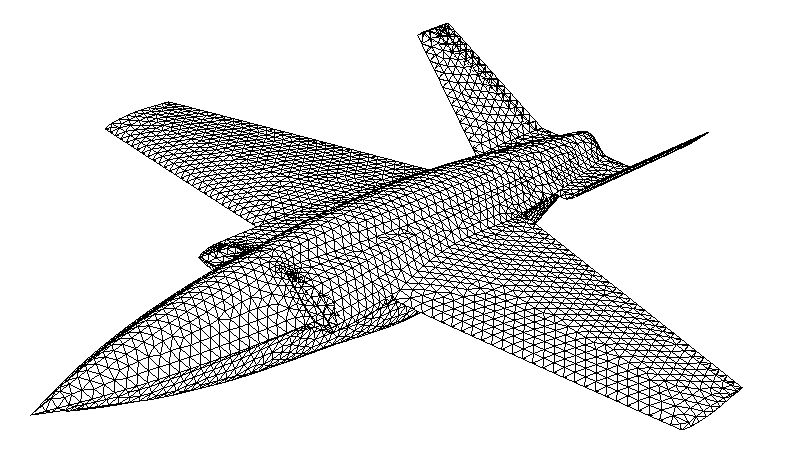
\includegraphics[width=10cm]{../isometric.png}
  };

  \begin{scope}[xslant=-0.2, yslant=-0.1, xscale=1, yscale=-0.38, rotate=-55]
    \draw[thick, cyan!60!blue!90!black, {Latex[length=4mm, width=3mm]}-, shift={(7.6, 0)}] (0,0) arc[start angle=0, end angle=180, radius=10cm] node[pos=0.5, yshift=-4mm] {\LARGE $\phi$};
  \end{scope}

  % \begin{scope}[x={(0.866cm,0.5cm)}, y={(0cm,1cm)}]
  %   \draw[thick, red] (0,0) arc[start angle=0, end angle=180, radius=1];
  % \end{scope}

  % \draw[thick, blue, domain=0:180, samples=100, variable=\t]
  %   plot ({cos(\t)}, {sin(\t)}, 0);

\end{tikzpicture}

\end{document}